We started talking about BRST transformations last time, given by the infinitesimal transformation
\begin{align*}
    \delta A_\mu^a &= \epsilon D_\mu^{ac} c^c\\
    \delta \psi &= ig \epsilon c^a t^a \psi\\
    \delta c^a &= -\frac{1}{2} g\epsilon f^{abc} c^b c^c\\
    \delta \bar c^a &= \epsilon B^a\\
    \delta B^a &= 0.
\end{align*}

In fact, the BRST transformation is nilpotent-- that is, the operator performed twice is zero. Let $S$ be the operator which represents the action of the BRST transformation on any field $\phi$ such that $\delta \phi = \epsilon s \phi$ (i.e. strip out the $\epsilon$). Thus
\begin{align}
    SA_\mu^a &= D^{ab}_\mu c^b\\
    Sc^a &= -\frac{1}{2} g f^{abc} c^b c^c,
\end{align}
and so on. One can show that $S^2\phi=0\implies S^2=0$.

Noether's theorem tells us that the symmetry of $\cL$ under $S$ implies the existence of a conserved current $j^\mu_\text{BRST}$ and an associated charge $Q_B$:
\begin{equation}
    Q_B =\int d^{d-1}x \,j^0_\text{BRST}(x)\text{ with }[Q_B,H]=0.
\end{equation}
Thus $S^2=0 \implies Q_B^2=0$.
%why?

Now $Q_B$ divides the Hilbert space $\cH$ into subspaces-- there are \term{closed states}, i.e. those annihilated by $Q_B$ (in the kernel):
\begin{equation}
    Q_B \ket{\Psi}=0 \text{ for }\ket{\Psi}\in \cH_{\text{closed}}
\end{equation}
and exact states, i.e. states in the image of $Q_B$, i.e. $\ket{\Psi}\in \cH_\text{exact}$ if
\begin{equation}
    \ket{\Psi} = Q_B \ket{\Phi} \text{ for some }\ket{\Phi} =\in \cH.
\end{equation}
Note that $\cH_\text{exact} \subset \cH_\text{closed}$ since $Q_B \ket{\psi}_{\text{exact}}=Q^2_B \ket{\Phi}=0$.

Physical states are those in the quotient space $\cH_\text{closed}/\cH_\text{exact}$, which is called the \term{BRST cohomology}. This is equivalent to the idea that some states are ``pure gauge'' and therefore non-physical. A more detailed analysis (see Srednicki and also Weinberg) shows that e.g. only the two transverse polarizations of $A_\mu^a$ belong in $\cH_\text{phys}=\cH_\text{closed}/\cH_\text{exact}$.%
    \footnote{This might feel similar to the Gupta-Bleuler condition in QED. In fact, I believe the BRST condition on physical states is actually a bit stronger, in that it encompasses Gupta-Bleuler for Abelian theories but also excludes some spurious states which we could not have gotten rid of with Gupta-Bleuler alone. For more details, see \url{https://physics.stackexchange.com/questions/383127/brst-cohomology-and-gupta-bleuler}}

\subsection*{One-loop renormalization}
Let us take our Lagrangian
\begin{equation}
    \cL= \frac{1}{2} (F_{\mu\nu}^a)^2 + \bar \psi(\slashed{D} +m)\psi + \frac{1}{2\xi} (\p^\mu A_\mu^a)^2 + \bar c \p^\mu D_\mu c.
\end{equation}
We can write down Feynman rules for such a theory:
\begin{itemize}
    \item Fermions are a solid directed line with propagator
    \begin{equation}
        \frac{1}{i\slashed{p}+m}\delta^{ij}=-\frac{i\slashed{p}-m}{p^2+m^2}\delta^{ij},
    \end{equation}
    where $ij$ are spinor indices.
    \item Gauge bosons are a curly line with propagator
    \begin{equation}
        \frac{1}{k^2} \paren{\delta^{\mu\nu} -(1-\xi) \frac{k^\mu k^\nu}{k^2}} \delta^{ab}.
    \end{equation}
    Note that gauge bosons have both generator indices (i.e. color indices) $ab$ as well as Lorentz indices $\mu\nu$.
    \item Ghosts get a dashed line with
    \begin{equation}
        \frac{\delta^{ab}}{q^2}.
    \end{equation}
    These have only generator indices $ab$.
\end{itemize}
We have interactions from the covariant derivative term and the field tensors,
\begin{align}
    D_\mu &= \p_\mu -ig A_\mu^a t^a\\
    F_{\mu\nu}^a &= \p_\mu A_\nu^a - \p_\nu A_\mu^a + g f^{abc} A_\mu^b A_\nu^c.
\end{align}
From the $gf^{abc}(\p_\mu A_\nu^a) A_\mu^b A_\nu^c$ term in the Lagrangian, we get a three-point gauge vertex,
\begin{center}
    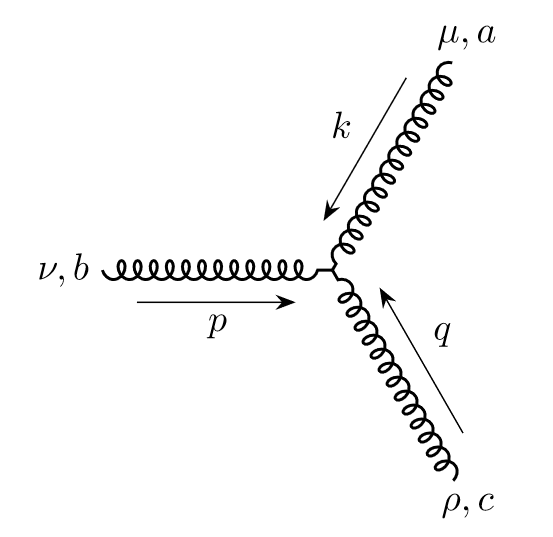
\includegraphics[scale=0.75]{2019/03/20190309_3pointgauge.PNG}
\end{center}
associated to an interaction
\begin{equation}
    gf^{abc} \bkt{
        \delta^{\mu\nu} (k-p)^\rho +\delta^{\nu\rho} (p-q)^\mu + \delta^{\rho\nu}(q-k)^\nu
    }.
\end{equation}
From the $(f^{abc}A_\mu^b A_\nu^c)(f^{ade}A_\mu^d A_\nu^e)$ term, we get a four-point gauge vertex,
\begin{center}
    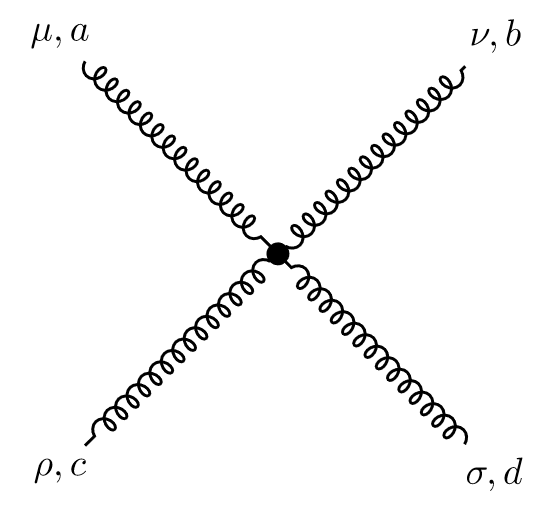
\includegraphics[scale=0.75]{2019/03/20190309_4pointgauge.PNG}
\end{center}
corresponding to a bunch of delta functions,
\begin{equation}
    -g^2 \bkt{f^{abc} f^{cde}(\delta^{\mu\rho} \delta^{\nu\sigma}-\delta^{\mu\sigma} \delta^{\nu\rho}) +f^{acd} f^{bde} (\delta^{\mu\nu}\delta^{\rho\sigma}-\delta^{\mu\sigma} \delta^{\nu\rho} + f^{ade}f^{bce} (\delta^{\mu\nu} \delta^{\rho\sigma} - \delta^{\mu\rho} \delta^{\nu\sigma}).
    }
\end{equation}
There are also the usual sorts of interactions between different kinds of particles-- there's a three point 2-fermion-gauge boson interaction
\begin{center}
    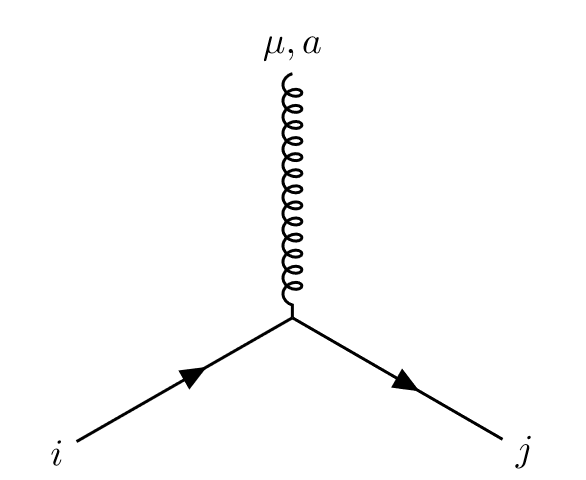
\includegraphics[scale=0.75]{2019/03/20190309_gluontwofermion.PNG}
\end{center}
with an amplitude 
\begin{equation}
    -ig \gamma^\mu t_{ij}^a
\end{equation}
and a three-point interaction between a gauge boson and two ghosts
%diagram
with an amplitude
\begin{equation}
    -g f^{abc} p^\mu.
\end{equation}

\subsection*{Vacuum polarization}
There are five diagrams we must consider in computing the vacuum polarization, i.e. corrections to the gauge boson propagator. There is a fermion loop, two gauge boson loops, a ghost loop, and a counterterm, as shown in Fig. \ref{fig:vacuumpolarization}.
\begin{figure}
    \centering
    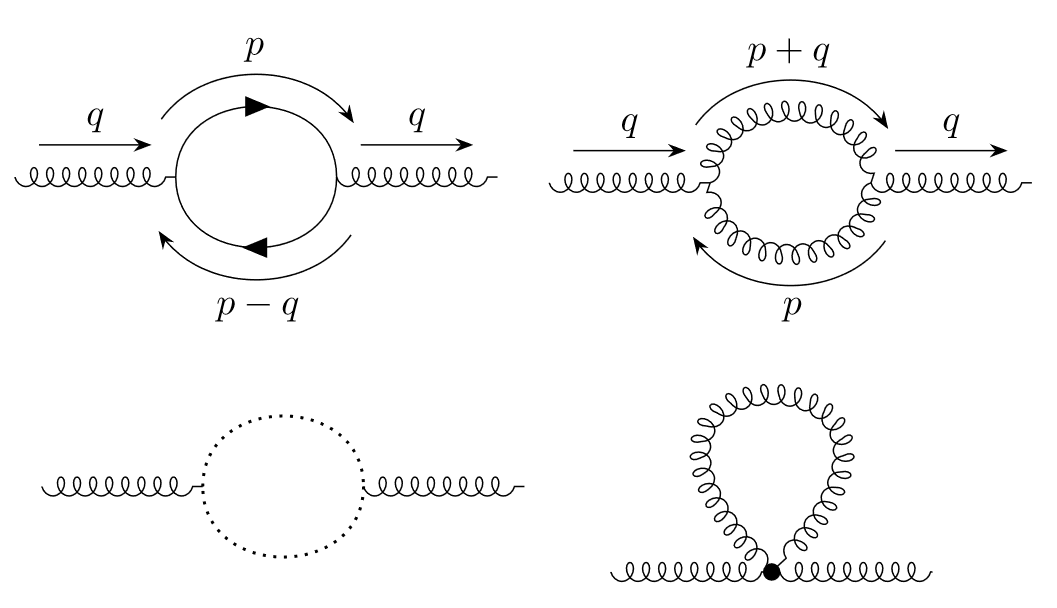
\includegraphics{2019/03/20190309_vacuumpolarization.PNG}
    \caption{Four of the diagrams which contribute to vacuum polarization. Clockwise from upper left: the fermion loop, the gluon loop with two 3-point vertices, the gluon loop with one 4-point vertex, and the ghost loop. The counterterm diagram is not shown-- we will determine what the value of the counterterm must be based on the sum of these four.}
    \label{fig:vacuumpolarization}
\end{figure}
We can calculate the amplitude of the fermion loop diagram as in QED. Applying the Feynman rules, it is
\begin{equation}
    M_F^{ab \mu\nu} = -\Tr(t^a t^b)(-g)^2 \mu^\epsilon \int \frac{d^d p}{(2\pi)^d} \frac{1}{(p-q)^2+m^2} \frac{1}{p^2+m^2} \times \Tr \set*{(-i\slashed{p}+m)\gamma^\mu [-i(\slashed{p}+\slashed{q})+m]\gamma^\mu}.
\end{equation}
Note that fermions transform under the fundamental representation so that $\Tr (t^a t^b)= \frac{1}{2} \delta^{ab}$, and in general $\Tr(t^a t^b)=C(r) \delta^{ab}$. These numerical factors $C(r)$s are called \term{Casimirs}-- they are related to the particular representation one works in. Thus our amplitude becomes
\begin{equation}
    M_F^{ab \mu\nu} = -\delta^{ab}(q^2 \delta^{\mu\nu}-  q^\mu q^\nu) C(r) \frac{g^2}{2\pi^2} \int_0^1 dx \, x(1-x) \paren{\frac{2}{\epsilon} -\gamma +\log \frac{4\pi \mu^2}{\Delta}}
\end{equation}
where $\Delta= m^2+ q^2x(1-x)$ and the $d^dp$ integral is identical to the QED case.

The gauge boson loops are somewhat similar. Working in Feynman gauge, $\xi=1$, the propagator is rather nicer (it is simply $\frac{1}{k^2}\delta^{\mu\nu}\delta^{ab}$) and we can immediately write down the amplitude
\begin{equation}
    \frac{g^2 \mu^\epsilon}{2} \int \frac{d^dp}{(2\pi)^d} \frac{1}{p^2(p+q)^2} f^{acd} f^{bcd} N^{\mu\nu},
\end{equation}
where $f^{acd}f^{bcd}=C_2(G)\delta^{ab}$ in terms of another Casimir and
\begin{equation}
    N^{\mu\nu}=\bkt{\delta^{\mu\rho}(q-p)^\sigma +\delta^{\rho\sigma}(2p+q)^\mu +\delta^{\sigma \mu}(-p - 2q)^\rho}\times
    \bkt{\delta^{\nu \rho}(p-q)^\sigma + \delta^{\rho\sigma}(-2p-q)^\nu + \delta^{\nu\rho}(p+2q)^\sigma
    }
\end{equation}

Using Feynman's trick, we rewrite the integral over the propagators in the nice form
\begin{equation}
    \int_0^1 dx \frac{1}{(P^2+\Delta)^2}
\end{equation}
where $\Delta=x(1-x)q^2$ and $P=p+xq$. Thus
\begin{align*}
    M_S^{ab \mu\nu} ={}& \frac{g^2 C_2(G)}{(4\pi)^{d/2}} \delta^{ab} \int_0^1 dx \frac{1}{\Delta^{2-d/2}} \times \left\{
        \Gamma(1-\frac{d}{2}) \delta^{\mu\nu} q^2 [\frac{3}{2}(d-1)x (1-x)] \right.\\
        &\left.+ \Gamma(2-\frac{d}{2}) \delta^{\mu\nu} q^2 [\frac{1}{2} (2-x)^2+\frac{1}{2}(1+x)^2]
        -\Gamma(2-\frac{d}{2})q^\mu q^\nu [(1-\frac{d}{2})(1-2x)^2+(1+x)(2-x)]\right\}.
\end{align*}
To be clear, these numerical factors come from expanding out $N^{\mu\nu}$ in terms of $P$ and explicitly evaluating the integral over $P$, noting that expressions odd in $P$ will integrate to zero.